\documentclass[12pt,letterpaper]{article}
\usepackage[utf8]{inputenc}
\usepackage[spanish]{babel}
\usepackage{graphicx}
\usepackage{hyperref}
\usepackage[left=2cm,right=2cm,top=2cm,bottom=2cm]{geometry}
\usepackage{graphicx} % figuras
% \usepackage{subfigure} % subfiguras
\usepackage{float} % para usar [H]
\usepackage{amsmath}
%\usepackage{txfonts}
\usepackage{stackrel} 
\usepackage{multirow}
\usepackage{enumerate} % enumerados
\renewcommand{\labelitemi}{$-$}
\renewcommand{\labelitemii}{$\cdot$}
% \author{}
% \title{Caratula}
\begin{document}

% Fancy Header and Footer
% \usepackage{fancyhdr}
% \pagestyle{fancy}
% \cfoot{}
% \rfoot{\thepage}
%

% \usepackage[hidelinks]{hyperref} % CREA HYPERVINCULOS EN INDICE

% \author{}
\title{Caratula}

\begin{titlepage}
\begin{center}
\large{UNIVERSIDAD PRIVADA-DE-TACNA}\\
\vspace*{-0.025in}
\begin{figure}[htb]
\begin{center}

\includegraphics[width=8cm]{./Imagenes/logo}
\end{center}
\end{figure}
\vspace*{0.15in}
INGENIERIA DE SISTEMAS  \\

\vspace*{0.5in}
\begin{large}
TITULO:\\
\end{large}

\vspace*{0.1in}
\begin{Large}
\textbf{INFORME DE LABORATORIO No 02} \\
\end{Large}

\vspace*{0.3in}
\begin{Large}
\textbf{CURSO:} \\
\end{Large}

\vspace*{0.1in}
\begin{large}
INTELIGENCIA DE NEGOCIOS\\
\end{large}

\vspace*{0.3in}
\begin{Large}
\textbf{DOCENTE(ING):} \\
\end{Large}

\vspace*{0.1in}
\begin{large}
 Patrick Cuadros Quiroga\\
\end{large}

\vspace*{0.2in}
\vspace*{0.1in}
\begin{large}
Integrante: \\
\begin{flushleft}

Ronald Eduardo Ordoñez Quilli  		\hfill	(2015052821) \\
\end{flushleft}
\end{large}
\end{center}

\end{titlepage}


\tableofcontents % INDICE
\thispagestyle{empty} % INDICE SIN NUMERO
\newpage
\setcounter{page}{1} % REINICIAR CONTADOR DE PAGINAS DESPUES DEL INDICE

 \section{Actividad – Crear relaciones} 
Para crear los informes en Power BI Desktop, primero debe conectarse a los datos y después darles forma. Después podrá guardar los informes en el formato de archivos de Power BI Desktop, que es la extensión .pbix. Y también va a poder compartirlos. Puede hacerlo como cualquier otro archivo, pero sin duda como va a aprovechar todo su potencial será si lo comparte desde el servicio de Power Bi.
\begin{itemize}
	\item Conectarse a datos: normalmente son varios orígenes de datos.
	\item Dar forma a dichos datos: mediante las consultas que crean modelos de datos precisos.
	\item Crear informes: usando modelos que otros pueden aprovechar, compartir y usar como punto de partida.\\
\end{itemize} 

\begin{itemize}
	\item Resultado del Modelo en Power BI 
	\begin{center}
	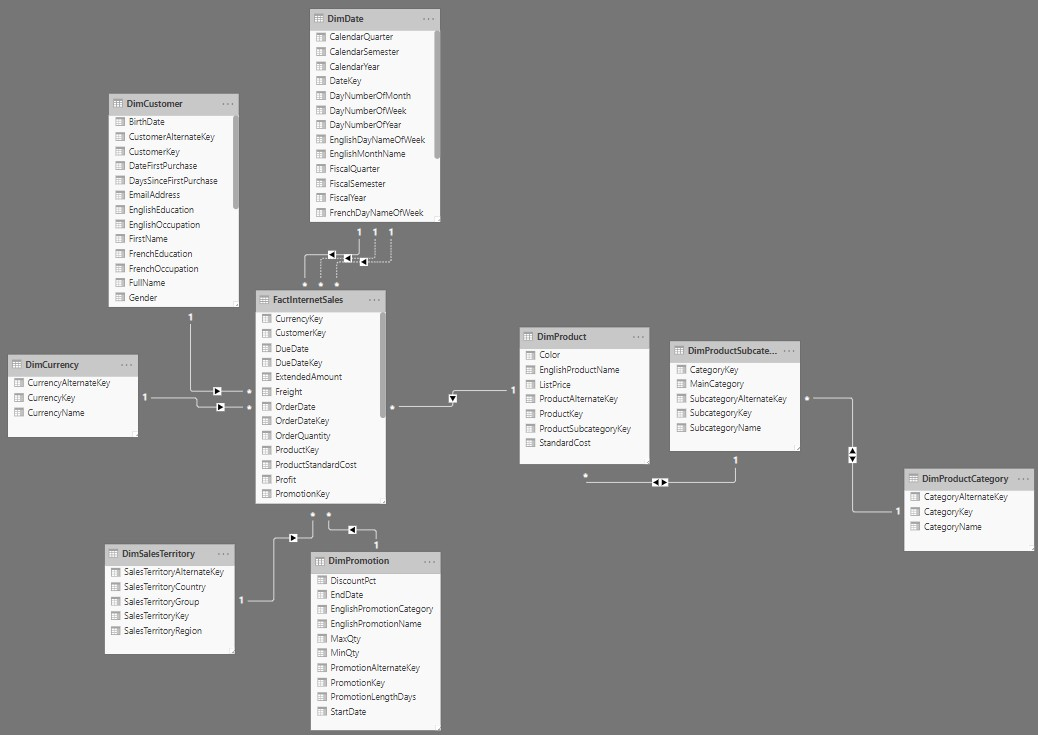
\includegraphics[width=16cm]{./Imagenes/imgpbi1} 
	\end{center}
\end{itemize} 
 \section{Actividad – Cálculos} 
Para crear los informes en Power BI Desktop, primero debe conectarse a los datos y después darles forma. Después podrá guardar los informes en el formato de archivos de Power BI Desktop, que es la extensión .pbix. Y también va a poder compartirlos. Puede hacerlo como cualquier otro archivo, pero sin duda como va a aprovechar todo su potencial será si lo comparte desde el servicio de Power Bi.
\begin{itemize}
	\item Conectarse a datos: normalmente son varios orígenes de datos.
	\item Dar forma a dichos datos: mediante las consultas que crean modelos de datos precisos.
	\item Crear informes: usando modelos que otros pueden aprovechar, compartir y usar como punto de partida.\\
\end{itemize} 

\begin{itemize}
	\item Resultado de cálculos en PowerBI
	\begin{center}
	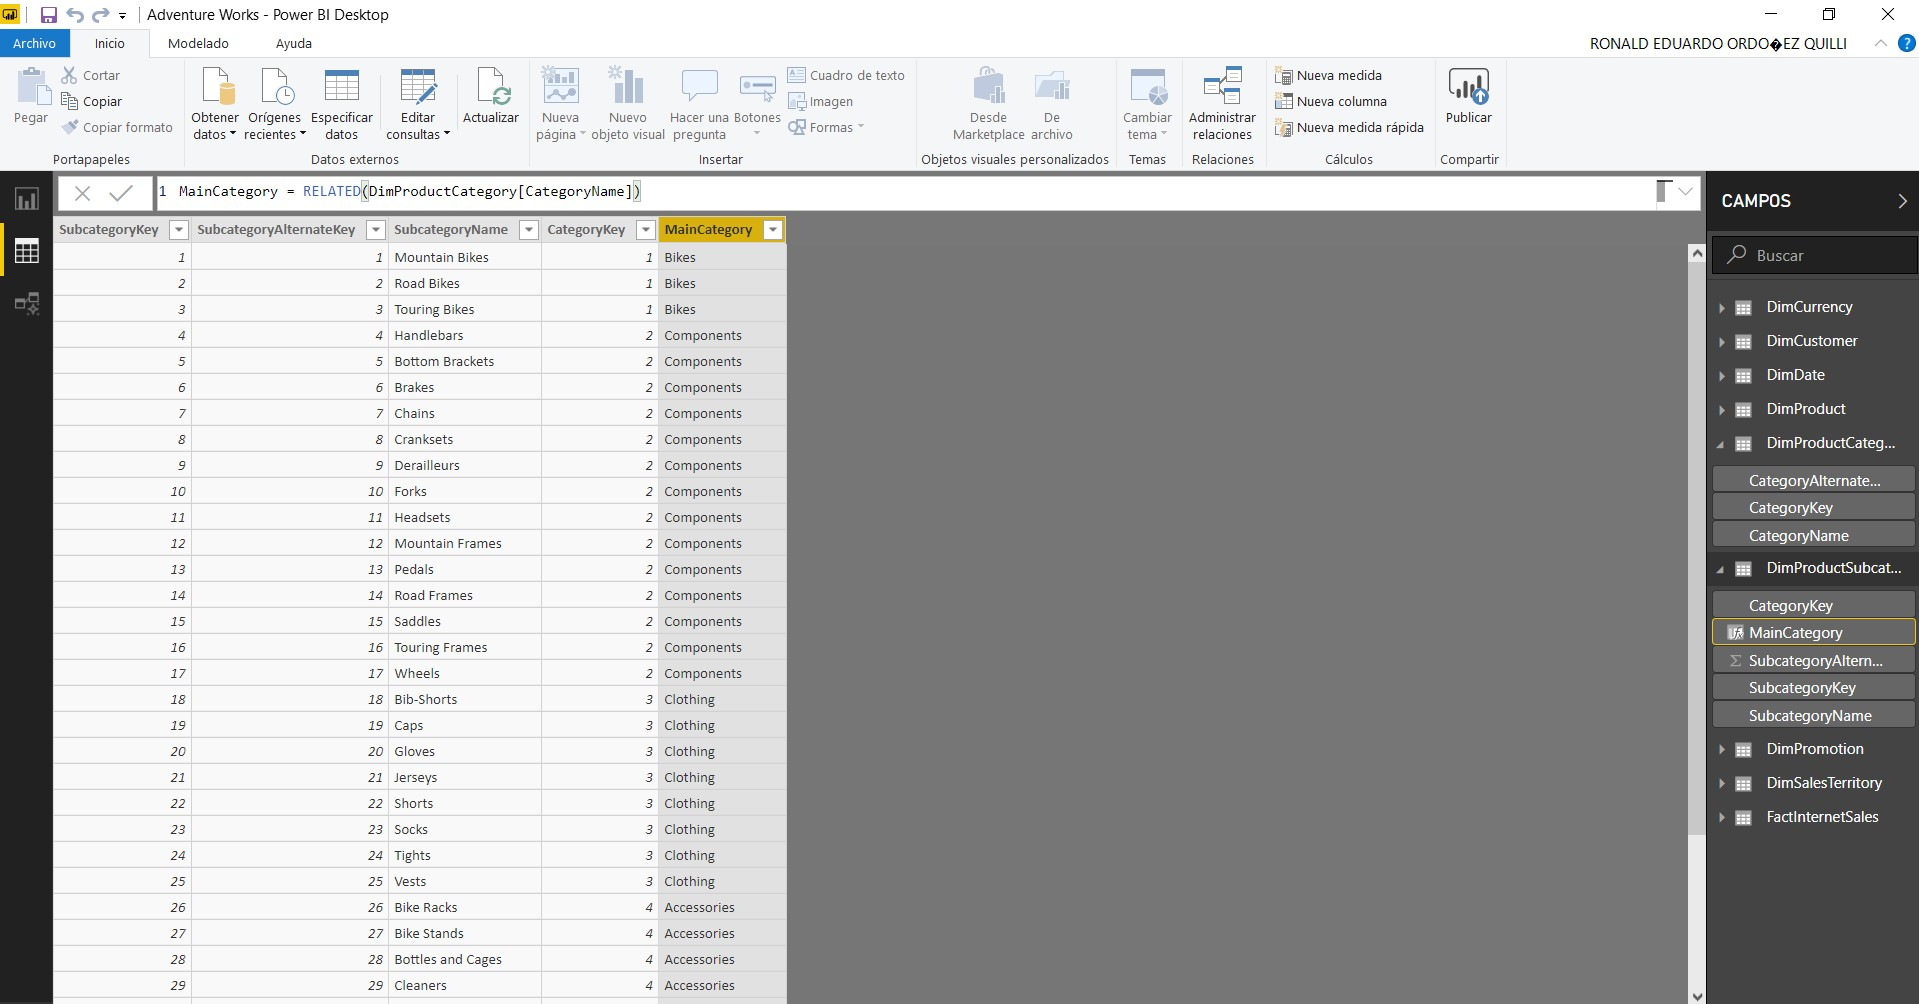
\includegraphics[width=16cm]{./Imagenes/imgpbi3} 
	\end{center}
	\begin{center}
	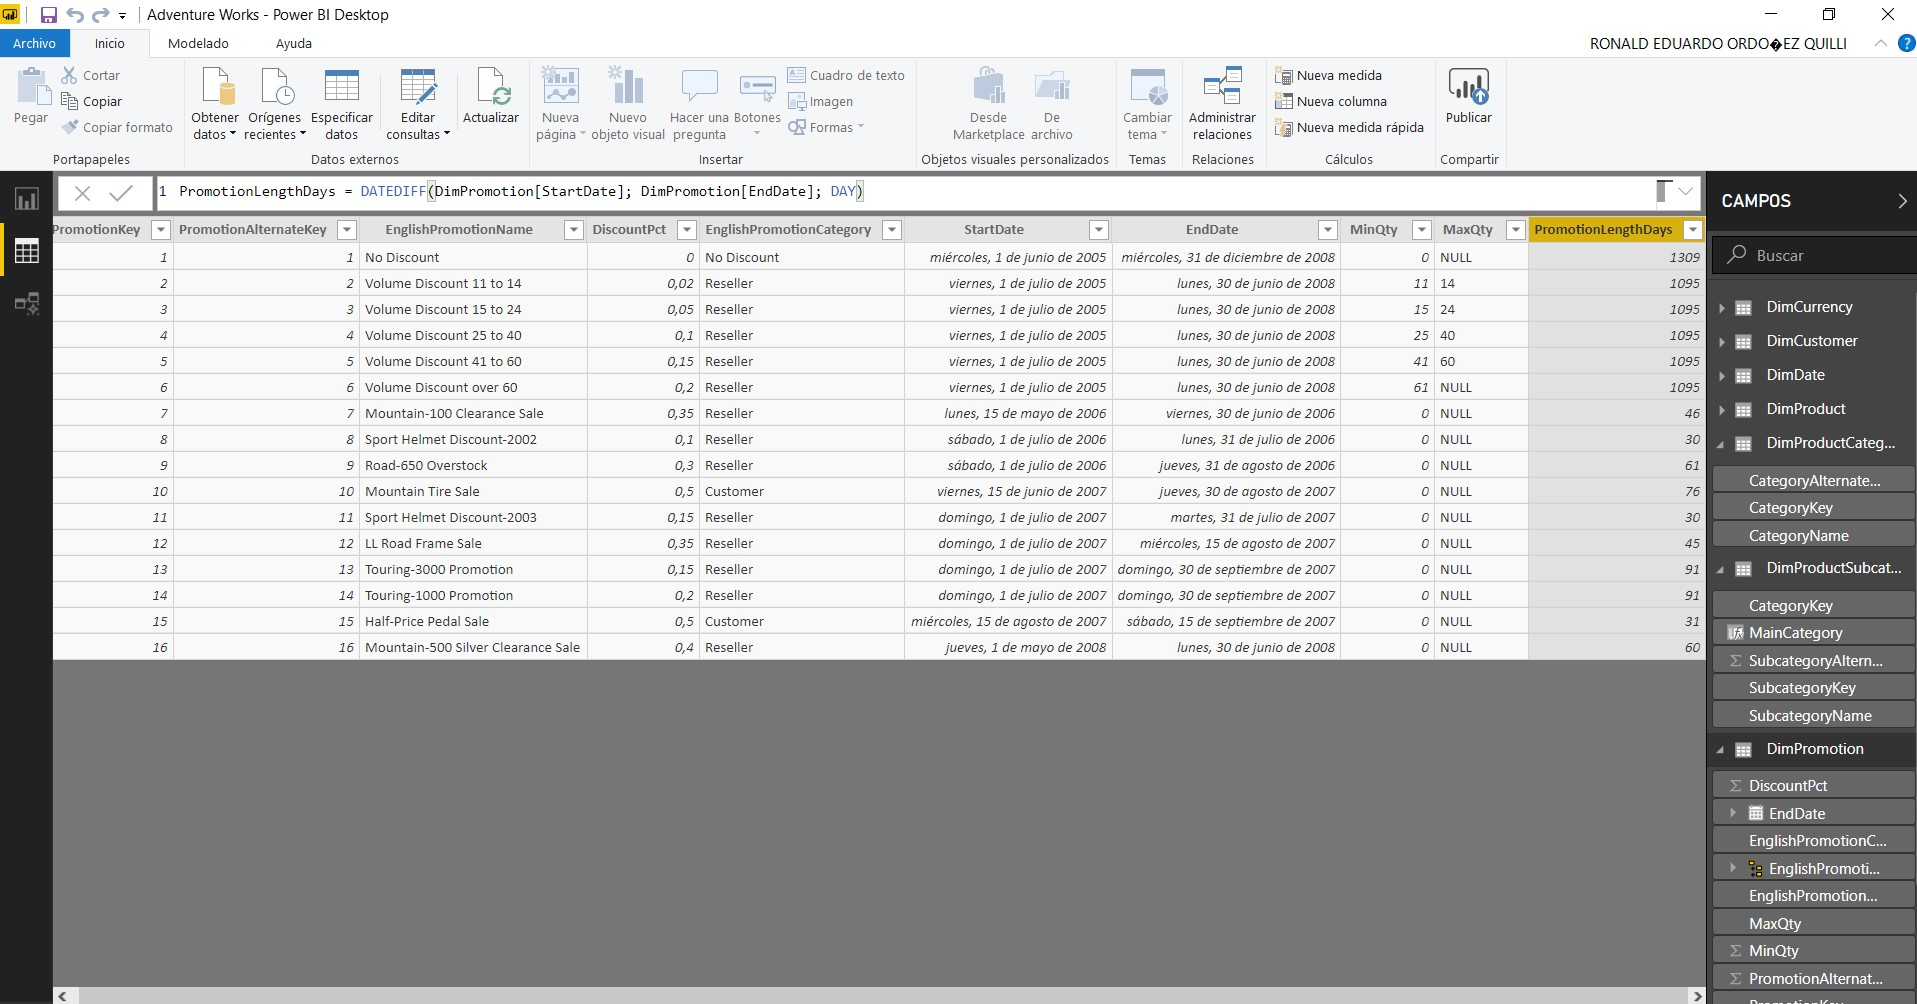
\includegraphics[width=16cm]{./Imagenes/imgpbi4} 
	\end{center}
	\begin{center}
	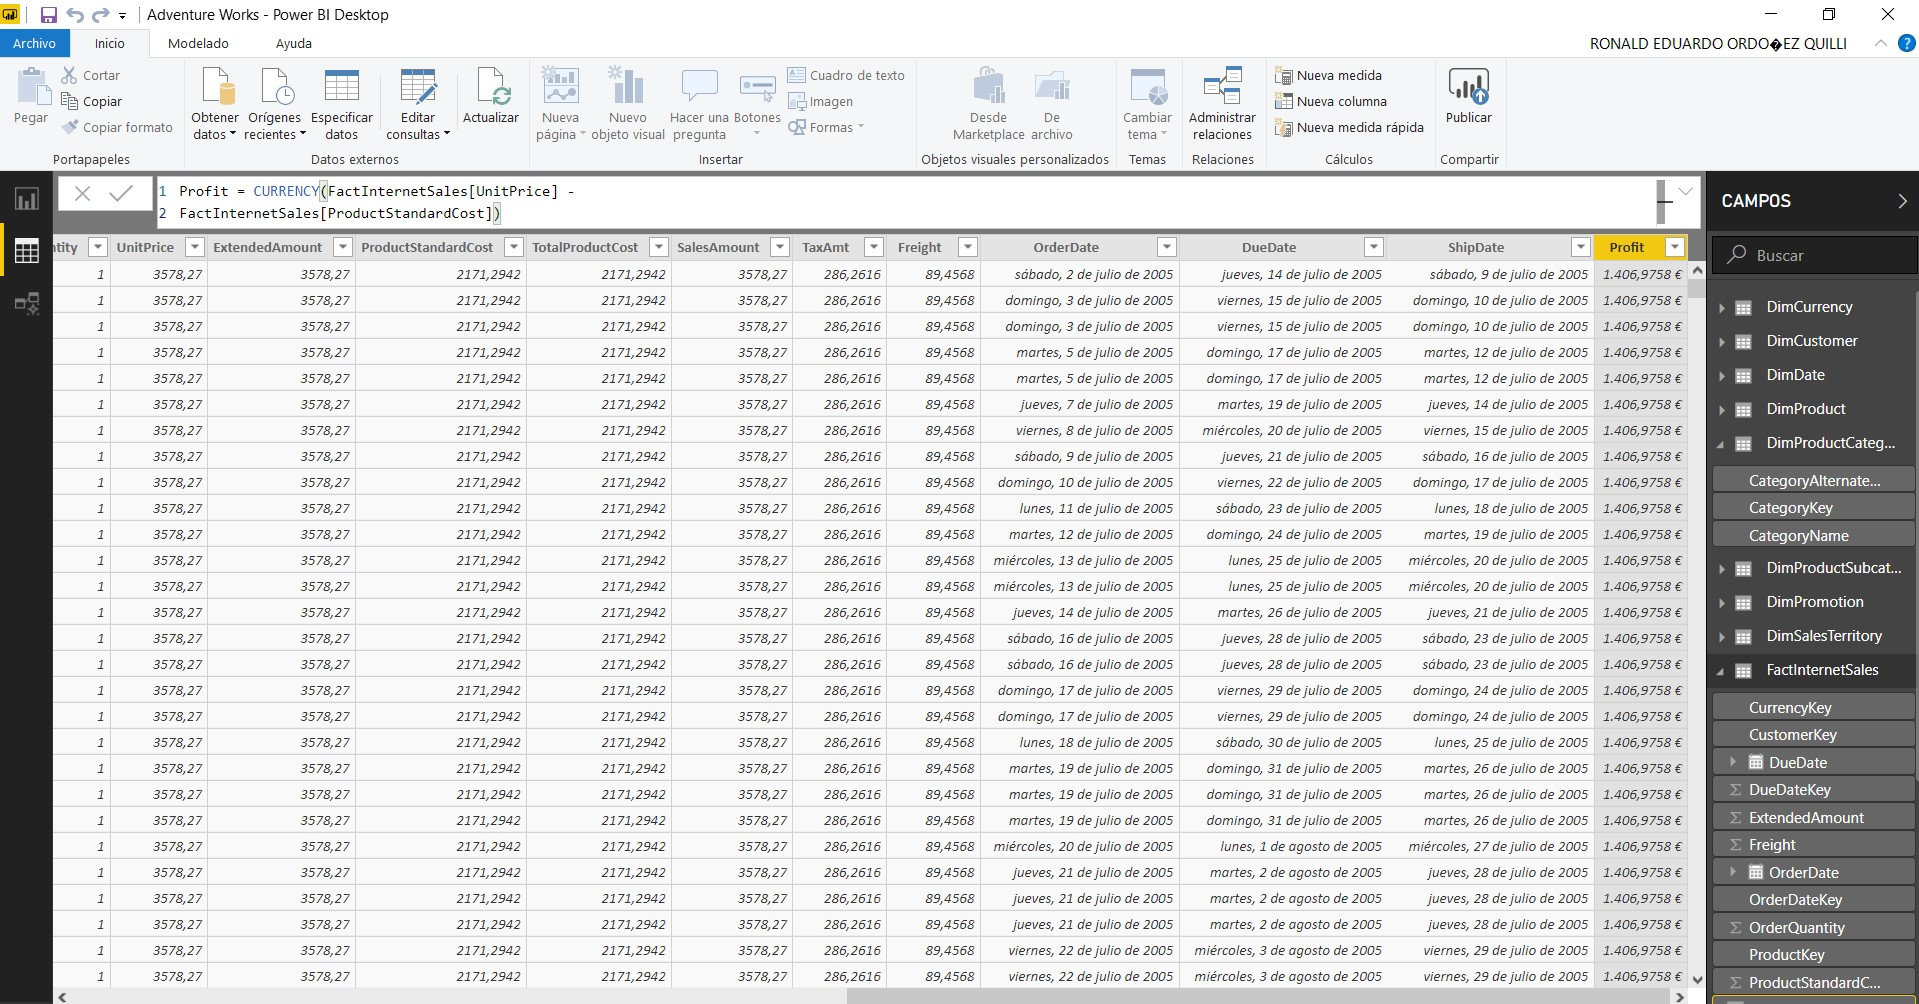
\includegraphics[width=16cm]{./Imagenes/imgpbi5} 
	\end{center}
	\item Informe en PowerBI
	\begin{center}
	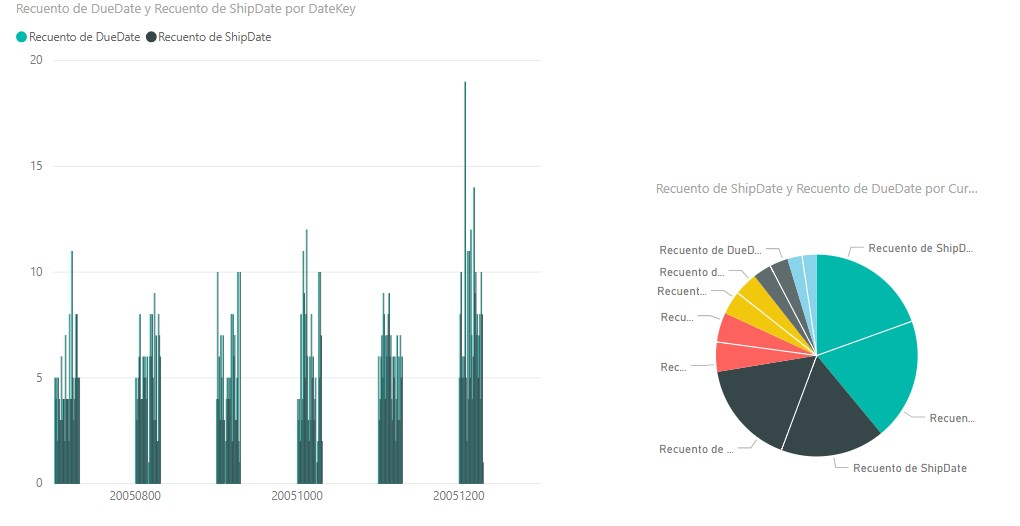
\includegraphics[width=16cm]{./Imagenes/imgpbi2} 
	\end{center}

Ruta del informe en el Power BI
\\
\url{https://app.powerbi.com/groups/me/reports/1a5e9816-31a8-46e2-b401-47d6bfac7293?ctid=b6b466ee-468d-4011-b9fc-fbdcf82ac90a} 
\end{itemize} 
\end{document}
